\section{Results}
(The figure doesn't show up in the preview but do show up if you export to pdf. Also these are generated in the 'paper plots' notebook; do not edit by hand.)

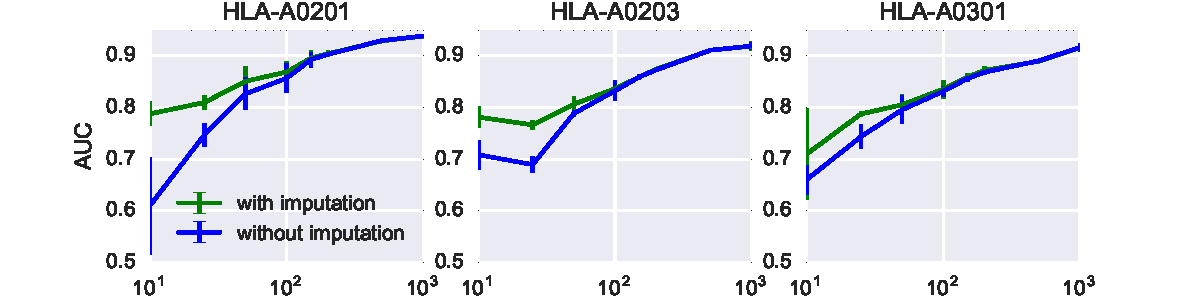
\includegraphics{figures/impute_comparison.pdf}


\begin{table}[h]
\begin{tabular}{llll}
\toprule
{} &              auc &               f1 &              tau \\
\midrule
mhcflurry ensemble &           0.9325 &           0.7847 &  \textbf{0.5865} \\
mhcflurry single   &           0.9313 &           0.7831 &           0.5843 \\
netmhc             &           0.9323 &  \textbf{0.8072} &           0.5863 \\
netmhcpan          &  \textbf{0.9326} &           0.7996 &           0.5814 \\
smmpmbec_cpp       &           0.9213 &           0.7903 &           0.5649 \\
\bottomrule
\end{tabular}

\caption{Performance on BLIND with equal weight given to each measurement}
\end{table}

\begin{table}[h]
\begin{tabular}{llll}
\toprule
{} &              auc &               f1 &              tau \\
\midrule
mhcflurry ensemble &           0.9103 &           0.6635 &           0.4890 \\
mhcflurry single   &           0.9095 &           0.6551 &           0.4874 \\
netmhc             &           0.9091 &           0.6790 &           0.4872 \\
netmhcpan          &  \textbf{0.9115} &  \textbf{0.6902} &  \textbf{0.4927} \\
smmpmbec_cpp       &           0.8933 &           0.6555 &           0.4661 \\
\bottomrule
\end{tabular}

\caption{Performance on BLIND with equal weight given to each allele (52 alleles)}
\end{table}

\begin{table}[h]
\begin{tabular}{llll}
\toprule
{} &              auc &               f1 &              tau \\
\midrule
mhcflurry ensemble &  \textbf{0.9117} &           0.6913 &  \textbf{0.5015} \\
mhcflurry single   &           0.9109 &           0.6873 &           0.4998 \\
netmhc             &           0.9086 &           0.7174 &           0.4984 \\
netmhcpan          &           0.9095 &  \textbf{0.7202} &           0.4994 \\
smmpmbec_cpp       &           0.8931 &           0.6964 &           0.4765 \\
\bottomrule
\end{tabular}

\caption{Performance on BLIND for alleles with at least 500 training observations (44 alleles)}
\end{table}

\begin{table}[h]
\begin{tabular}{llllllll}
\toprule
allele &        HLA-A2602 &        HLA-A2603 &        HLA-B0803 &        HLA-B1509 &        HLA-B1503 &           H-2-KD &        HLA-B0802 \\
\midrule
train size         &              202 &              205 &              217 &              346 &              429 &              452 &              487 \\
test size          &              413 &              312 &              234 &              466 &              165 &              229 &              509 \\
mhcflurry ensemble &           0.9288 &           0.9096 &           0.9521 &           0.8877 &           0.8388 &           0.7905 &           0.9828 \\
mhcflurry single   &           0.9284 &           0.9062 &           0.9580 &           0.8864 &           0.8354 &           0.7898 &           0.9826 \\
netmhc             &           0.9316 &           0.8902 &           0.9684 &           0.9012 &           0.8648 &           0.8153 &  \textbf{0.9899} \\
netmhcpan          &  \textbf{0.9578} &  \textbf{0.9343} &           0.9523 &  \textbf{0.9229} &  \textbf{0.8701} &  \textbf{0.8192} &           0.9896 \\
smmpmbec_cpp       &           0.9430 &           0.8432 &  \textbf{0.9733} &           0.8946 &           0.8394 &           0.7537 &           0.9872 \\
\bottomrule
\end{tabular}

\caption{AUC scores on BLIND dataset for alleles with $\lt 500$ training examples}
\end{table}
